\documentclass[11pt]{beamer}
\usetheme{Montpellier}
\usefonttheme[onlymath]{serif}
\usecolortheme{rose}

\usepackage{tikz} \usepackage{graphicx} \usepackage{algorithm} \usepackage[noend]{algpseudocode} \usepackage{caption}
\usepackage{amsmath} \usepackage{pgfplots} \usepackage{float}

\usetikzlibrary{shapes.geometric, arrows}

\setbeamertemplate{navigation symbols}{}
\setbeamerfont{page number in head/foot}{size=\fontsize{9}{11}}
\setbeamertemplate{footline}[frame number]
\setbeamertemplate{section in toc}{\inserttocsectionnumber.~\inserttocsection}

\author{Glenn Galvizo}
\title{Efficient Determination of an Optimal Microsatellite Mutation Model}
%\subtitle{\scriptsize A Coalescent-based Approximate Bayesian Markov Chain Monte Carlo approach.}
\institute{University of Hawaii at Manoa}

% Has to be in the preamble...
\usetikzlibrary{calligraphy}

\begin{document}
    \begin{frame}
        \titlepage
    \end{frame}

	\section{Introduction}\label{sec:i}
	\begin{frame}
		\frametitle{Overview}
        \tableofcontents
	\end{frame}

	\begin{frame}
		\frametitle{How much do we know about human history?}
	\end{frame}

	\subsection{Problem Statement}\label{subsec:ps}
	\begin{frame}
		\frametitle{Research Goal: Efficient Parameter Estimation}
        \begin{enumerate}
            \item What are the best microsatellite mutation parameters?
        \end{enumerate}
	\end{frame}

	\section{Microsatellites}\label{sec:mi}
	\subsection{DNA Variation: Tandem Repeats}\label{subsec:dvtr}
    \begin{frame}
        \frametitle{What is a microsatellite?}
        \begin{definition}[Microsatellite]
            A \emph{microsatellite} is a short sequence in DNA that is repeated in tandem.
        \end{definition} \bigskip

        \begin{columns}
            \begin{column}{0.4\textwidth}
                \begin{itemize}
                    \item Interested in number of repeats.
                    \item Represent variation in humans.
                    \item More variable than SNP marker~\cite{gemayelJunkVariableTandemRepeats2012}.
                \end{itemize}
            \end{column}
            \begin{column}{0.6\textwidth}
                \begin{equation*}
                    \begin{aligned}
                         \ldots &\text{AACG}\textbf{ATATATATATAT}\text{GGCTA} \ldots \\
                         \ldots &\text{AACG}\textbf{ATATATATAT}\text{GGCTA} \ldots \\
                         \ldots &\text{AACG}\textbf{ATATATAT}\text{GGCTA} \ldots \\
                         \ldots &\text{AACG}\textbf{ATATAT}\text{GGCTA} \ldots \\
                         \ldots &\text{AACG}\textbf{ATAT}\text{GGCTA} \ldots
                    \end{aligned}
                \end{equation*}
            \end{column}
        \end{columns}
    \end{frame}

    \subsection{Microsatellite Data}\label{subsec:md}
    \begin{frame}
        \frametitle{What data are we working with?} \bigskip
        \centering{\input{include/floats/frequency-graphs-present.tex}}
        \bigskip
        \newline
        \centering{\emph{Populations of \text{GATA} microsatellite variations, interested in frequency of a
        repeat length.}}
    \end{frame}

    \subsection{Mutation}\label{subsec:mm}
    \begin{frame}
        \frametitle{How do microsatellites mutate?}
        \begin{columns}
            \begin{column}{0.5\textwidth}
                \begin{itemize}
                    \item SMM: Mutate up one, down one, or not at all~\cite{sainudiinMicrosatelliteMutationModels2004}.
                        \medskip
                    \item Three parameters: $c, u, d$ \medskip.
                    \item Upward mutation = $\frac{d}{u}\ell + c$. \medskip
                    \item Downward mutation = $d\ell$. \medskip
                    \item Focal bias = intersection of both lines.
                \end{itemize}
            \end{column}
            \begin{column}{0.6\textwidth}
                \medskip

                \centering{\pgfplotsset{compat=1.5}
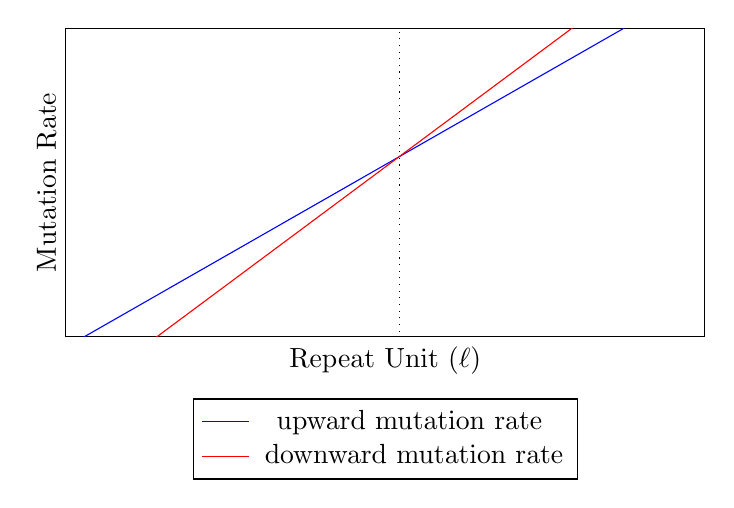
\begin{tikzpicture}
    \begin{axis}[
    width=0.8\linewidth, height=5.5cm,
    ylabel={Mutation Rate}, ymin=0.01, ymax=0.03,
    xlabel={Repeat Unit ($\ell$)}, xmin=2, xmax=13,
    xtick={0, 2, 4, 6, 8, 10, 12, 14, 16, 18, 20, 22, 24, 26},
    samples=100, no markers, enlargelimits=false, legend style={at={(0.5,-0.2)},anchor=north},
    domain=0:25, ticks=none
    ]
        \addplot {(0.0028/1.3)*x + 0.005};
        \addlegendentry{upward mutation rate};

        \addplot {0.0028*x};
        \addlegendentry{\vspace*{1em} downward mutation rate};

        \addplot+[mark=very thick, black, dotted, forget plot] coordinates {(7.7381, 0) (7.7381, 0.05)};
    \end{axis}
\end{tikzpicture}} \newline
            \end{column}
        \end{columns}
    \end{frame}

%    \subsection{Human Dataset}\label{subsec:hm}
%    \begin{frame}
%        \frametitle{What dataset are we using?}
%        \begin{itemize}
%            \item Using GATA sequences.
%            \item 330 different populations from ALFRED (the ALelle FREquency Database).
%            \item
%        \end{itemize}
%    \end{frame}

    \section{Methodology}\label{sec:m}
	\subsection{Coalescent Simulation}\label{subsec:c}
    \begin{frame}
        \frametitle{How do we simulate evolution?}
        \begin{columns}
            \begin{column}{0.5\textwidth}
                We construct a evolutionary tree!
                \begin{enumerate}
                    \item Given sample size $n$, parameters $c, u, d$. \medskip
                    \item Construct random tree with $n$ leaves and common ancestor. \medskip
                    \item Randomly choose repeat unit of common ancestor. \medskip
                    \item Mutate children from ancestors until leaves are reached.
                \end{enumerate}
            \end{column}
            \begin{column}{0.5\textwidth}
                \centering{\input{include/floats/coalescent-tree-present.tex}}
            \end{column}
        \end{columns}
    \end{frame}

	\subsection{Markov Chain Monte Carlo (MCMC)}\label{subsec:mcmc}
    \begin{frame}
        \frametitle{How do we choose which parameters are best?}
        \begin{definition}[Markov Chain Monte Carlo]
            A \emph{Markov Chain Monte Carlo} (MCMC) method is a technique to draw samples from a distribution.
        \end{definition}
        \begin{columns}
            \begin{column}{0.5\textwidth}
                \begin{enumerate}
                    \item Given data to compare to and starting parameters. \medskip
                    \item Generate several populations using parameters. \medskip
                    \item Compare this to observed data. Compute the likelihood $p_x$. \medskip
                    \item  $p_x$
                \end{enumerate}
            \end{column}
            \begin{column}{0.6\textwidth}
                \medskip
                \centering{\pgfplotsset{compat=1.5}
\pgfmathdeclarefunction{gauss}{2}{%
  \pgfmathparse{1/(#2*sqrt(2*pi))*exp(-((x-#1)^2)/(2*#2^2))}%
}

\begin{tikzpicture}
    \begin{axis}[
    width=0.8\linewidth, height=5.6cm,
    ylabel={Likelihood}, ymax=0.3,
    xlabel={Parameter}, xmin=0, xmax=10,
    samples=100, no markers, enlargelimits=false, legend style={at={(0.5,-0.35)},anchor=north},
    domain=0:25, ticks=none
    ]
    \addplot [very thick,cyan!50!black] {gauss(5,1.5)};
    \end{axis}
\end{tikzpicture}} \newline
            \end{column}
        \end{columns}
    \end{frame}

    \section{Results}\label{sec:r}
    \subsection{Posterior Distribution}\label{subsec:pd}
    \begin{frame}
        \frametitle{What are our results?}
    \end{frame}

    \subsection{Trace Plot}\label{subsec:tp}
    \begin{frame}
        \frametitle{How do we know if this is correct?}
    \end{frame}

    \section{Conclusion}\label{sec:c}
    \begin{frame}
        
    \end{frame}

    \begin{frame}
        \frametitle{Acknowledgments}
        \begin{columns}
            \begin{column}{0.4\textwidth}
                \begin{itemize}
                    \item Dr. Floyd Reed \bigskip
                    \item Undergraduate Showcase \bigskip
                    \item The Audience \bigskip
                \end{itemize}
            \end{column}
            \begin{column}{0.5\textwidth}
                \centering{\includegraphics[scale=0.08]{images/undergraduate-showcase-logo.png}}
                \bigskip \bigskip
                \newline
                \centering{\includegraphics[scale=0.07]{images/uh-logo.png}}
            \end{column}
        \end{columns}
    \end{frame}

    \begin{frame}
        \frametitle{References}
        \scriptsize
        \bibliographystyle{abbrv}
        \bibliography{include/references}
    \end{frame}

    \begin{frame}
        \centering{\huge{Questions? :-)}}
    \end{frame}

\end{document}